\chapter*{Введение}
\addcontentsline{toc}{chapter}{Введение}

\textbf{Расстояние Левенштейна}, или редакционное расстояние,~--- метрика cходства между двумя строковыми последовательностями. Чем больше расстояние, тем более различны строки. Для двух одинаковых последовательностей расстояние равно нулю. По сути, это минимальное число односимвольных преобразований (удаления, вставки или замены), необходимых, чтобы превратить одну последовательность в другую.

\textbf{Расстояние Дамерау~---~Левенштейна} является модификацией расстояния Левенштейна~--- это мера разницы двух строк символов, определяемая как минимальное количество операций вставки, удаления, замены и транспозиции (перестановки двух соседних символов), необходимых для перевода одной строки в другую. К операциям вставки, удаления и замены символов, определённых в расстоянии Левенштейна добавлена операция транспозиции (перестановки) символов.

Расстояние Левенштейна активно используется для исправления ошибок в словах, поиска дубликатов текстов, сравнения геномов и прочих полезных операций с символьными последовательностями.

\textbf{Целью} данной лабораторной работы является получить навыки динамического программирования на задаче поиска редакционных расстояний.

Необходимо выполнить следующие \textbf{задачи}:
\begin{enumerate}
    \item Изучить алгоритмы поиска расстояния Левенштейна и Дамерау~---~Левенштейна.
    \item Разработать и реализовать алгоритмы поиска редакционных расстояний.
    \item Выполнить замеры затрат реализаций алгоритмов по памяти.
    \item Выполнить замеры затрат реализаций алгоритмов по процессорному времени.
    \item Провести сравнительных анализ двух нерекурсивных алгоритмов.
\end{enumerate}


\chapter{Аналитическая часть}

\section{Расстояние Левенштейна}
Расстояние Левенштейна~--- метрика, измеряющая по модулю разность между двумя последовательностями символов. Она определяется как минимальное количество односимвольных операций (а именно вставки, удаления, замены), необходимых для превращения одной последовательности символов в другую. В общем случае, операциям, используемым в этом преобразовании, можно назначить разные цены \cite{analysis-lev-damlev}.

\begin{enumerate}
    \item \textbf{I}~(от англ. insert)~--- вставка символа ($w(\lambda, b) = 1$);
    \item \textbf{R}~(от англ. replace)~--- замена символа ($w(a, b) = 1$, $a \neq b$);
    \item \textbf{D}~(от англ. delete)~--- удаление символа ($w(a, \lambda) = 1$).
    \item \textbf{M}~(от англ. match)~--- совпадение символа ($w(a, a) = 0$);
\end{enumerate}

Также рассмотрим функцию $D(i, j)$: ее значением является
редакционное расстояние между строками $S_1[1...i]$ и $S_2[1...j]$.

Расстояние Левенштейна между двумя строками $S_{1}$ и $S_{2}$ (длиной $M$ и $N$ соответственно) рассчитывается по следующей рекуррентной формуле:

\begin{equation}
	\label{eq:L}
	D(i, j) =
	\begin{cases}
		0, &\text{i = 0, j = 0}\\
		i, &\text{j = 0, i > 0}\\
		j, &\text{i = 0, j > 0}\\
		min \begin{cases}
			D(i, j - 1) + 1,\\
			D(i - 1, j) + 1,\\
			D(i - 1, j - 1) +  m(S_{1}[i], S_{2}[j]), \\
		\end{cases}
		&\text{i > 0, j > 0}
	\end{cases}
\end{equation}
где сравнение символов строк $S_1$ и $S_2$ рассчитывается таким образом:
\begin{equation}
	\label{eq:m}
	m(a, b) = \begin{cases}
		0 &\text{если a = b,}\\
		1 &\text{иначе.}
	\end{cases}
\end{equation}

\section{Расстояние Дамерау~---~Левенштейна}
Расстояние Дамерау~---~Левенштейна между двумя строками, состоящими из конечного числа символов~--- это минимальное число операций вставки, удаления, замены одного символа и транспозиции двух соседних символов, необходимых для перевода одной строки в другую.

Расстояние Дамерау~---~Левенштейна определятся следующей рекуррентной формуле:

\begin{multline}
    D(m, n) =\\ =
    \begin{cases}
        0, &\text{i = 0, j = 0}\\
        i, &\text{j = 0, i > 0}\\
        j, &\text{i = 0, j > 0}\\
        \min
        \begin{cases}
            D(i, j - 1) + 1,\\
            D(i - 1, j) + 1,\\
            D(i - 1, j - 1),\\
            D(i - 2, j - 2) + 1,
        \end{cases} 
        &\begin{aligned}
            & \text{если $i, j > 1$}, \\
            & S_{1}[i] = S_{2}[j - 1], \\
            & S_{1}[i - 1] = S_{2}[j],
        \end{aligned} \\
        \min
        \begin{cases}
            D(i - 1, j) + 1, \\
            D(i, j - 1) + 1, \\
            D(i - 1, j - 1) + \text{m}(S_1[i], S_2[j])
        \end{cases} &\text{иначе.}
    \end{cases}
    \label{eqn:recur-damlev}
\end{multline}

\section*{Вывод}
В данном разделе были рассмотрены алгоритмы нахождения расстояния Левенштейна и Дамерау~---~Левенштейна.
\clearpage

\chapter{Конструкторская часть}
В данном разделе будут приведены схемы алгоритмов нахождения расстояний Левенштейна и Дамерау~---~Левенштейна, описание используемых типов данных и структуры программного обеспечения.

\section{Требования к программному обеспечению}

К программе предъявлен ряд функциональных требований:

\begin{itemize}
    \item наличие интерфейса для выбора действий;
    \item возможность ввода строк с клавиатуры;
    \item возможность обработки строк, состоящих из символов латинского алфавита или арабских цифр;
    \item возможность произвести замеры процессорного времени работы реализованных алгоритмов поиска расстояний Левенштейна и Дамерау~---~Левенштейна;
\end{itemize}

\section{Требования к вводу}

К допустимому вводу представлены следующие ограничения:

\begin{enumerate}
    \item На вход реализованным алгоритмам подаются две строки;
    \item Строки могут включать символы латинского алфавита или арабских цифр;
    \item Буквы нижнего и верхнего регистра считаются разными символами;
\end{enumerate}

\section{Разработка алгоритмов}


На рисунке \ref{fig:lev-iter} представлена схема матричного алгоритма поиска расстояния Левенштейна.

На рисунке \ref{fig:dam-lev-iter} приведена схема матричной реализации алгоритма поиска расстояния Дамерау~---~Левенштейна.

На рисунке \ref{fig:dam-lev-rec} представлена его рекурсивная реализация.

На рисунке \ref{fig:dam-lev-rec-cache} показана рекурсивная реализация алгоритма нахождения расстояния Дамерау~---~Левенштейна с использованием матрицы-кэша.
\begin{figure}[h]
	\centering
	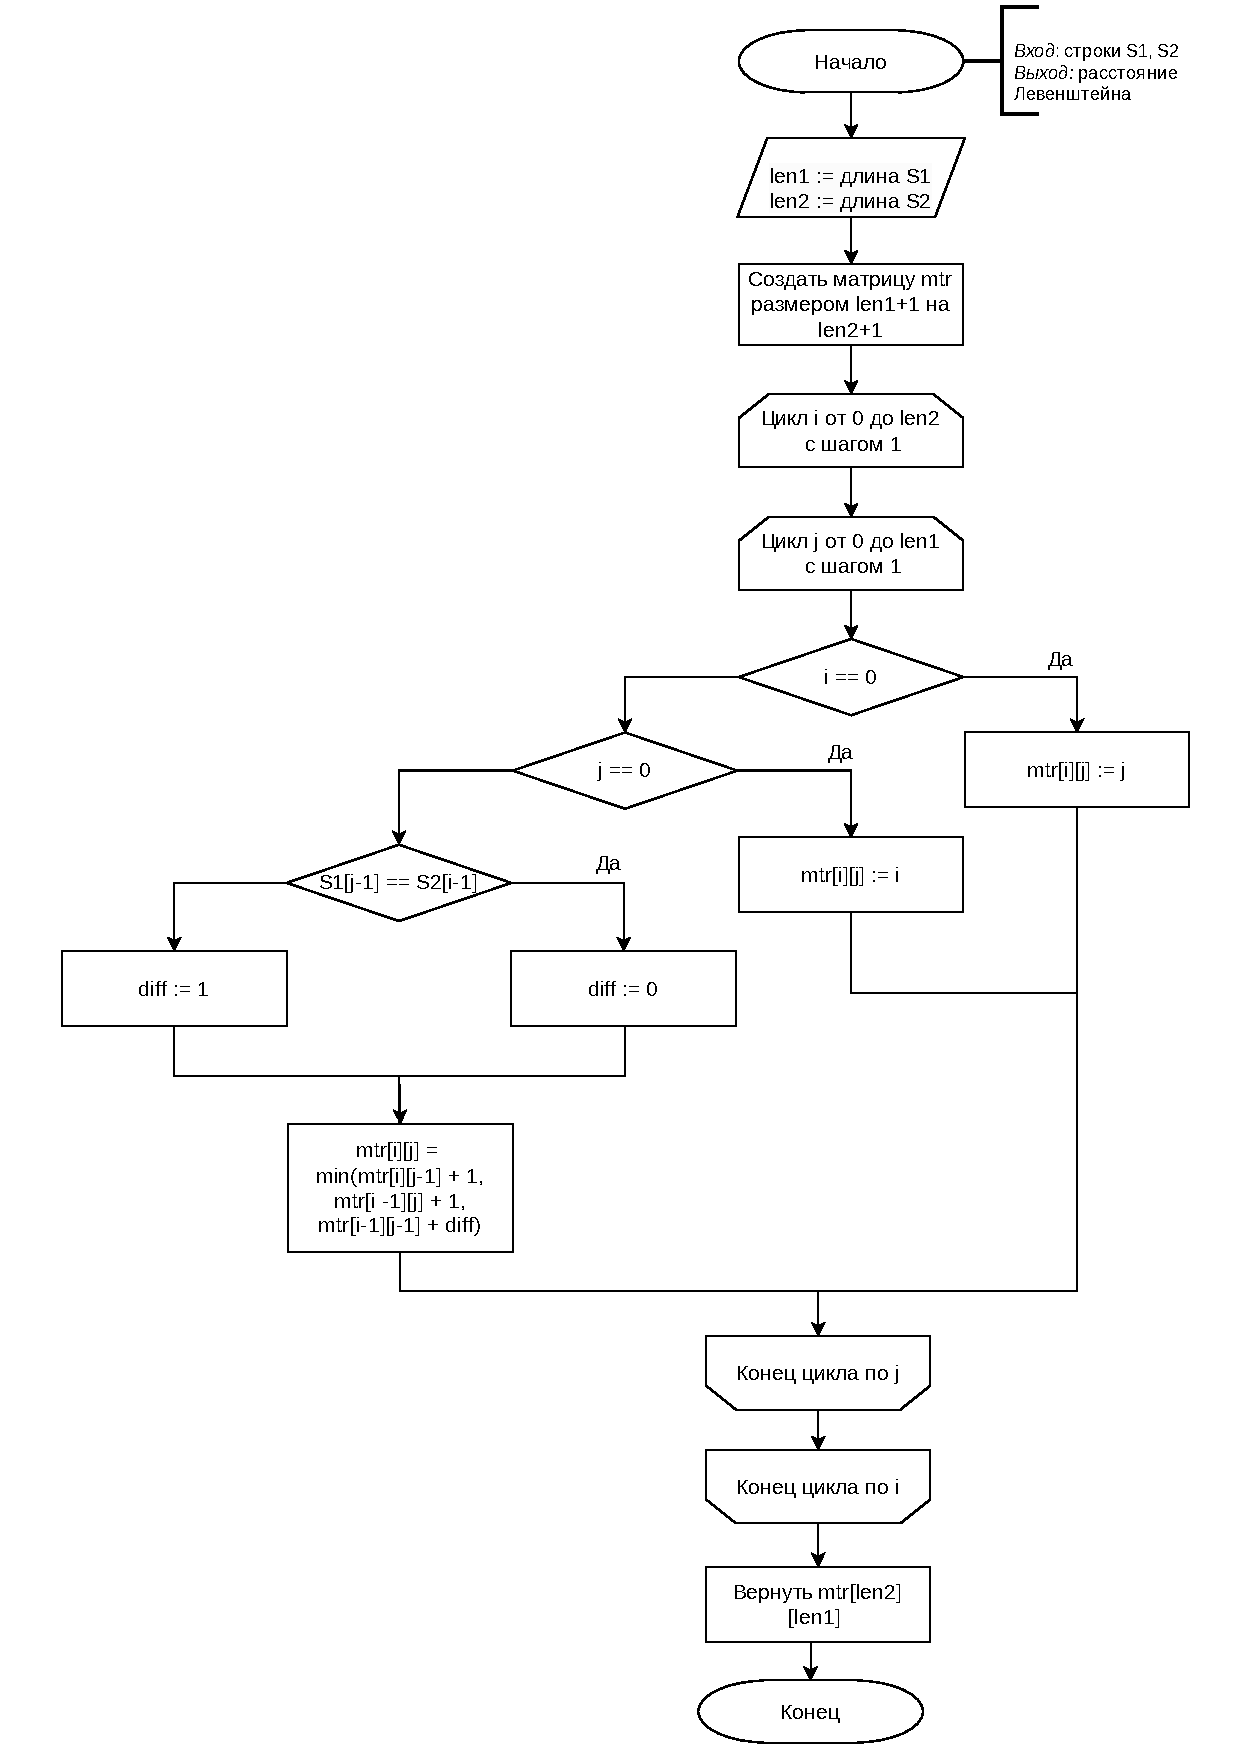
\includegraphics[height=0.7\textheight, page=1]{algo-scheme.pdf}
	\caption{Схема нерекурсивного алгоритма нахождения расстояния Левенштейна}
	\label{fig:lev-iter}
\end{figure}

\clearpage

\begin{figure}[h]
	\centering
	\includegraphics[height=0.9\textheight, page=2]{algo-scheme.pdf}
	\caption{Схема нерекурсивного алгоритма нахождения расстояния Дамерау~---~Левенштейна}
	\label{fig:dam-lev-iter}
\end{figure}

\clearpage

\begin{figure}[h]
	\centering
	\includegraphics[height=0.9\textheight, page=3]{algo-scheme.pdf}
	\caption{Схема рекурсивного алгоритма нахождения расстояния Дамерау~---~Левенштейна}
	\label{fig:dam-lev-rec}
\end{figure}

\clearpage

\begin{figure}[h]
	\centering
	\includegraphics[height=0.9\textheight, page=4]{algo-scheme.pdf}
	\caption{Схема алгоритма вызова рекурсивного алгоритма нахождения расстояния Дамерау~---~Левенштейна с кешированием}
	\label{fig:dam-lev-rec-cache-decor}
\end{figure}

\begin{figure}[h]
	\centering
	\includegraphics[height=0.9\textheight, page=5]{algo-scheme.pdf}
	\caption{Схема рекурсивного алгоритма нахождения расстояния Дамерау~---~Левенштейна с кешированием}
	\label{fig:dam-lev-rec-cache}
\end{figure}

\clearpage


\section{Описание используемых типов данных}

При реализации алгоритмов будут использованы следующие типы данных:

\begin{itemize}
    \item \textit{строка}~--- массив \texttt{символьного типа};
    \item \textit{матрица}~--- двумерный массив \texttt{целочисленного типа}.
\end{itemize}

\section*{Вывод}
\addcontentsline{toc}{section}{Вывод}

В данном разделе на основе теоретических данных были перечислены требования к ПО и построены схемы реализуемых алгоритмов на основе данных, полученных на этапе анализа.

\clearpage

\chapter{Технологическая часть}
В данном разделе будут приведены средства реализации, листинг кода и функциональные тесты.

\section{Средства реализации}

В качестве языка программирования, используемого при написании данной лабораторной работы, был выбран C++ \cite{cpp-lang}, так как в нем имеется контейнер \texttt{std::string}, представляющий собой массив символов \texttt{char}, и библиотека \texttt{<ctime>} \cite{ctime}, позволяющая производить замеры процессорного времени.

В качестве среды для написания кода был выбран \textit{Visual Studio Code} за счет того, что она предоставляет функционал для проектирования, разработки и отладки ПО.

\section{Сведения о модулях программы}

Данная программа разбита на следующие модули:

\begin{itemize}
    \item \texttt{main.cpp}~--- точка входа программы, пользовательское меню;
    \item \texttt{algo}~--- модуль с реализациями алгоритмов поисков расстояний;
    \item \texttt{measurement}~--- модуль с реализаций функции подсчёта затрачиваемого времени;
\end{itemize}

\clearpage

\section{Реализация алгоритмов}

Далее будет представлена реализация алгоритмов поиска редакционных растояний:

\begin{lstlisting}[caption=Матричный алгоритм поиска расстояния Левенштейна]
int matrix_lev_temp(const char* str1,const char* str2, int width, int height)
{
    int diff;

    int** matrix = new int*[height];
    for (int i = 0; i < height; ++i)
        matrix[i] = new int[width];

    for(int i = 0; i < width; i ++)
    {
        matrix[0][i] = i;
    }
    for(int i = 1; i < height; i ++)
    {
        matrix[i][0] = i;
    }

    for(int i = 1; i < height; i ++)
    {
        for(int j = 1; j < width; j ++)
        {
            int minval = min(matrix[i][j - 1], matrix[i - 1][j]);
            minval ++;
            minval = min(minval, matrix[i - 1][j - 1] + int(str1[j] != str2[i]));

            matrix[i][j] = minval;
        }
    }

    if(MODE == MODE_INTERACTIVE)
        print_matrix(matrix, width, height);

    diff = matrix[height - 1][width - 1];

    for (int i = 0; i < height; ++i)
        delete[] matrix[i];    
    delete[] matrix;

    return diff;
}
\end{lstlisting}

\clearpage

\begin{lstlisting}[caption=Матричный алгоритм поиска расстояния Дамерау~---~Левенштейна]
int matrix_dam_lev_temp(const char* str1,const char* str2, int width, int height)
{
    int diff;

    int** matrix = new int*[height];
    for (int i = 0; i < height; ++i)
        matrix[i] = new int[width];


    for(int i = 0; i < height; i ++)
    {
        for(int j = 0; j < width; j ++)
        {
            matrix[i][j] = 0;  
        }
    }  

    for(int i = 0; i < width; i ++)
    {
        matrix[0][i] = i;
    }
    for(int i = 1; i < height; i ++)
    {
        matrix[i][0] = i;
    }

    for(int i = 1; i < width; i ++)
    {
            int minval = min(matrix[i][0], matrix[i - 1][1]);
            minval ++;
            minval = min(minval, matrix[i - 1][0] + int(str1[1] != str2[i]));
            matrix[i][1] = minval;
    }

    for(int j = 1; j < height; j ++)
    {
            int minval = min(matrix[1][j - 1], matrix[0][j]);
            minval ++;
            minval = min(minval, matrix[0][j - 1] + int(str1[j] != str2[1]));
            matrix[1][j] = minval;
    }

    for(int i = 2; i < height; i ++)
    {
        for(int j = 2; j < width; j ++)
        {
            int minval = min(matrix[i][j - 1], matrix[i - 1][j]);
            minval ++;
            minval = min(minval, matrix[i - 1][j - 1] + int(str1[j] != str2[i]));
            if(str1[j] == str2[i - 1] && str1[j - 1] == str2[i])
            {
                minval = min(minval, matrix[i - 2][j - 2] + 1);
            }
            matrix[i][j] = minval;  
        }
    }  

    if(MODE == MODE_INTERACTIVE)
        print_matrix(matrix, width, height);  

    diff = matrix[height - 1][width - 1];

    for (int i = 0; i < height; ++i)
        delete[] matrix[i];    
    delete[] matrix;

    return diff;
}
\end{lstlisting}
\clearpage

\begin{lstlisting}[caption=Рекурсивный алгоритм поиска расстояния Дамерау~---~Левенштейна]
int recurs_dam_lev_temp(const char*str1, const char*str2, int length1, int length2)
{
    if (length1 == 0)
        return length2;
    if (length2 == 0)
        return length1;

    int change = 0;
    int res = 0;
    if (str1[length1 - 1] != str2[length2 - 1])
        change = 1;

    res = min(recurs_dam_lev_temp(str1, str2, length1, length2 - 1) + 1,
                min(recurs_dam_lev_temp(str1, str2, length1 - 1, length2) + 1,
                    recurs_dam_lev_temp(str1, str2, length1 - 1, length2 - 1) + change));

    if (length1 > 1 && length2 > 1 &&
        str1[length1 - 1] == str2[length2 - 2] &&
        str1[length1 - 2] == str2[length2 - 1])
        res = min(res, recurs_dam_lev_temp(str1, str2, length1 - 2, length2 - 2) + 1);
    return res;    
}
\end{lstlisting}
\clearpage
\begin{lstlisting}[caption=Рекурсивный алгоритм поиска расстояния Дамерау~---~Левенштейна с кэшированием (реализация)]
int hash_dam_lev_temp(const char*str1, const char*str2, int **matrix, int width, int height)
{
    if (height == 0)
        return matrix[height][width] = width;
    if (width == 0)
        return matrix[height][width] = height;

    int change = 0;
    if (str1[height - 1] != str2[width - 1])
        change = 1;


    matrix[height][width] = min(hash_dam_lev_temp(str1, str2, matrix, height, width - 1) + 1,
                    min(hash_dam_lev_temp(str1, str2, matrix, height - 1, width) + 1,
                        hash_dam_lev_temp(str1, str2, matrix, height - 1, width - 1) + change));

    if (height > 1 && width > 1 &&
        str1[height - 1] == str2[width - 2] &&
        str1[height - 2] == str2[width - 1])
        matrix[height][width] = min(matrix[height][width], hash_dam_lev_temp(str1, str2, matrix, height - 2, width - 2) + 1);

    return matrix[height][width];
}
\end{lstlisting}
\clearpage
\begin{lstlisting}[caption=Рекурсивный алгоритм поиска расстояния Дамерау~---~Левенштейна с кэшированием (оберточная функция)]
template <IsStr T>
int hash_dam_lev(const T& str1,const T& str2)
{

    size_t width = str1.length() + 1;
    size_t height = str2.length() + 1;

    int** matrix = new int*[height];
    for (int i = 0; i < height; i++)
        matrix[i] = new int[width];

    for (int i = 0; i < height; i++)
    {
        for (int j = 0; j < width; j++)
        {
                matrix[i][j] = 0;
        }
    }
    int diff = hash_dam_lev_temp(str1.c_str(), str2.c_str(), matrix, width - 1, height - 1);

    for (int i = 0; i < height; ++i)
        delete[] matrix[i];    
    delete[] matrix;

    return diff;

}
\end{lstlisting}
\clearpage
\section{Функциональные тесты}

В данном разделе будут представлены функциональные тесты, проверяющие работу алгоритмов поиска расстояний.

\begin{table}[ht]\centering
	\small
	\begin{center}
		\begin{threeparttable}
		\caption{Функциональные тесты}
		\label{tbl:func_tests}
		\begin{tabular}{|c|c|c|c|c|c|}
			\hline
			\multicolumn{2}{|c|}{\bfseries Входные данные}
			& \multicolumn{4}{c|}{\bfseries Расстояние и алгоритм} \\ 
			\hline 
			&
			& \multicolumn{1}{c|}{\bfseries Левенштейна} 
			& \multicolumn{3}{c|}{\bfseries Дамерау~---~Левенштейна} \\ \cline{3-6}
			
			\bfseries Строка 1 & \bfseries Строка 2 & \bfseries Итеративный & \bfseries Итеративный
			
			& \multicolumn{2}{c|}{\bfseries Рекурсивный} \\ \cline{5-6}
			& & & & \bfseries Без кеша & \bfseries С кешем \\
			\hline
			kitten & sitting & 4 & 4 & 4 & 4 \\
			\hline
			book & back & 2 & 2 & 2 & 2 \\
			\hline
			back & bakc & 2 & 1 & 1 & 1 \\
			\hline
			saturday & sunday & 3 & 3 & 3 & 3 \\
			\hline
			intention & inteniton & 2 & 1 & 1 & 1 \\
			\hline
		\end{tabular}	
		\end{threeparttable}
	\end{center}
\end{table}

\section*{Вывод}

Были реализованы алгоритмы Левенштейна (итеративно) и Дамерау~---~Левенштейна (итеративно, рекурсивно, рекурсивно с кэшированием).
Проведено тестирование реализованных алгортимов.

\clearpage

\chapter{Исследовательская часть}

\section{Технические характеристики}
Технические характеристики устройства, на котором выполнялись
замеры по времени:

\begin{itemize}
    \item Процессор: Intel Core i7 9750H 2.6 ГГц.
    \item Оперативная память: 16 ГБ.
    \item Операционная система: Kubuntu 22.04.3 LTS x86\_64 Kernel: 6.2.0-36-generic.
\end{itemize}

Во время проведения измерений времени ноутбук был подключен к сети электропитания и был нагружен только системными приложениями.

\section{Демонстрация работы программы}

На рисунке \ref{fig:img_prog} показан пример работы с программой.


\begin{figure}[ht!]
	\centering
	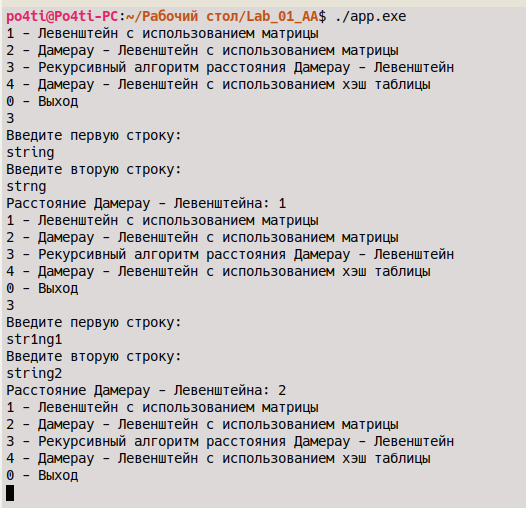
\includegraphics[width=170mm]{img/img_prog.png}
	\caption{Демонстрация работы программы.\label{overflow}}
	\label{fig:img_prog}
	\end{figure}


\clearpage

\section{Временные характеристики}

В связи с экспоненциальным ростом затрачиваемого времени рекурсивными алгоритмами, верхняя граница длин строк для тестирования таких алгоритмов ограничена до 10.

Итого, исследование временных характеристик реализованных алгоритмов производилось на строках длинами:

\begin{itemize}
    \item 1 -- 10 c шагом 1 для рекурсивных реализаций;
    \item 1 -- 200 c шагом 1 для нерекурсивных реализаций.
\end{itemize}

На рисунке \ref{fig:plotting_data1} показаны зависимости времени выполнения матричных реализаций алгоритмов Левенштейна и Дамерау~---~Левенштейна от длин входящих строк.

На рисунке \ref{fig:plotting_data2} показаны зависимости времени выполнения рекурсивных реализаций алгоритмов Левенштейна и Дамерау~---~Левенштейна от длин входящих строкк.


\begin{figure}[H]
    \includesvg[width=1.0\textwidth]{img/plotting_data1.svg}
    \caption{Результат измерений времени работы (в мс) нерекурсивных реализаций алгоритмов поиска расстояний Левенштейна и Дамерау~---~Левенштейна}
    \label{fig:plotting_data1}
\end{figure}

\begin{figure}[H]
    \includesvg[width=1.0\textwidth]{img/plotting_data2.svg}
    \caption{Результат измерений времени работы рекурсивных реализаций алгоритма поиска расстояния Дамерау~---~Левенштейна}
    \label{fig:plotting_data2}
\end{figure}


\section{Характеристики по памяти}

Введем следующие обозначения:

\begin{itemize}
    \item $m$~--- длина строки $S_1$;
    \item $n$~--- длина строки $S_2$;
    \item $\text{size}(v)$~--- функция, вычисляющая размер входного параметра $v$ в байтах;
    \item $char$~--- тип данных, используемый для хранения символа строки;
    \item $int$~--- целочисленный тип данных.
\end{itemize}

Теоретически оценим объем используемой памяти итеративной реализацией алгоритма поиска расстояния Левенштейна:

\begin{multline}
    M_{LevIter} = (m + 1) \cdot (n + 1) \cdot \text{size}(int) + (m + n) \cdot \text{size}(char) + \\
    + \text{size}(int**) + (m + 1) \cdot \text{size}(int*) + \\
    + 3 \cdot \text{size}(int) + 2 \cdot \text{size}(int)
\end{multline}
где $(m + 1) \cdot (n + 1) \cdot \text{size}(int)$~--- размер матрицы,
\newline $\text{size}(int**)$~--- размер указателя на матрицу,
\newline $(m + 1) \cdot \text{size}(int*)$~--- размер указателей на строки матрицы,
\newline $(m + n) \cdot \text{size}(char)$~--- размер двух входных строк,
\newline $2 \cdot \text{size}(int)$~--- размер переменных, хранящих длину строк,
\newline $3 \cdot \text{size}(int)$~--- размер дополнительных переменных.

Для алгоритма поиска расстояния Дамерау~---~Левенштейна теоретическая оценка объема используемой памяти идентична.

Произведем оценку затрат по памяти для рекурсивных реализаций алгоритма нахождения расстояния Дамерау~---~Левенштейна.

Рассчитаем объем памяти, используемой каждым вызовом функции поиска расстояния Дамерау~---~Левенштейна:
\begin{equation}
    M_{call} = (m + n) \cdot \text{size}(char) + 2 \cdot \text{size}(int) + 3 \cdot \text{size}(int) + 8
\end{equation}
где $(m + n) \cdot \text{size}(char)$~--- объем памяти, используемый для хранения двух строк,
\newline $2 \cdot \text{size}(int)$~--- размер двух входных строк,
\newline $3 \cdot \text{size}(int)$~--- размер дополнительных переменных,
\newline 8 байт~--- адрес возврата.

Максимальная глубина стека вызовов при рекурсивной реализации равна сумме длин входящих строк, поэтому максимальный расход памяти равен

\begin{equation}
    M_{DLRec} = (m + n) \cdot M_{call}
\end{equation}
где $m + n$~--- максимальная глубина стека вызовов,
\newline $M_{call}$~--- затраты по памяти для одного рекурсивного вызова.

Рекурсивная реализация алгоритма поиска расстояния Дамерау~---~Левенштейна с кэшированием для хранения промежуточных значений использует матрицу (кэш), размер которой можно рассчитать следующим образом:

\begin{multline}
	M_{cache} = (n + 1) \cdot (m + 1) \cdot \text{size}(int) +\\+ \text{size}(int **) + (m + 1) \cdot \text{size}(int *)
\end{multline}
где $(n + 1) \cdot (m + 1)$~--- количество элементов в кэше,
\newline $\text{size}(int **)$~--- размер указателя на матрицу,
\newline $(m + 1) \cdot \text{size}(int *)$~--- размер указателя на строки матрицы.

Таким образом, затраты по памяти для рекурсивного алгоритма нахождения расстояния Дамерау~---~Левенштейна с использованием кэша:

\begin{equation}
    M_{DLRecCache} = M_{DLRec} + M_{cache}
\end{equation}

\section{Вывод}

В результате исследования реализуемых алгоритмов по времени выполнения можно сделать следующие выводы:

\begin{enumerate}
    \item При небольших длинах строк (длина < 5 симв.) разница между временем выполнения нерекурсивных реализаций алгоритмов Левенштейна и Дамерау~---~Левенштейна незначительна.
    Однако, при увеличении длины обрабатываемых строк алгоритм поиска расстояния Дамерау~---~Левенштейна выполняется на порядок дольше, что связано с обработкой дополнительного условия о перестановке символов.
    \item Рекурсивная реализация алгоритма поиска расстояния Дамерау~---~Левенштейна с использованием кэша работает на порядок быстрее реализации поиска этого расстояния без кэширования.
    \item Время работы матричной и рекурсивной с кэшем реализаций алгоритма поиска расстояния Дамерау~---~Левенштейна приблизительно равны и выполняются на порядок быстрее в сравнении с рекурсивной реализацией поиска этого расстояния без кэширования.
\end{enumerate}

В результате исследования алгоритмов по затрачиваемой памяти можно сделать вывод о том, что итеративные алгоритмы и рекурсивный алгоритм с кэшированием требуют больше памяти по сравнению с рекурсивным без оптимизаций.
В реализациях, использующих матрицу, максимальный размер используемой памяти увеличивается пропорционально произведению длин строк, в то время как у рекурсивного алгоритма без кэширования объем затрачиваемой памяти увеличивается пропорционально сумме длин строк.

\chapter{Заключение}
В результате выполнения лабораторной работы для достижения этой цели были выполнены следующие задачи:
\begin{enumerate}
    \item описаны алгоритмы поиска расстояния Левенштейна и Дамерау~---~Левенштейна;
    \item разработаны и реализованы соответствующие алгоритмы;
    \item создано программное обеспечение, позволяющее протестировать реализованные алгоритмы;
    \item проведен сравнительный анализ процессорного времени выполнения реализованных алгоритмов:
    \begin{itemize}
        \item при малых длинах строк $(< 5)$ рекурсивные реализации с кешем и без для поиска расстояния Дамерау~---~Левенштейна имеют приблизительно одинаковое время работы, 
	    но с увеличением длины строки реализация без кеша выполняется на порядок дольше, поскольу не происходит повторное вычисление значений;
        \item разница между итеративными реализацими алгоритмов поиска расстояний Левенштейна и Дамерау~---~Левенштейна незначительна, и обусловлена она
        дополнительным условием на проверку равенства соседних символов для расстояния Дамерау~---~Левенштейна;
        \item итеративная реализация работает на порядок быстрее рекурсивной с кешем для поиска расстояния Дамерау~---~Левенштейна.
        \end{itemize}
    \item проведен сравнительный анализ затрачиваемой алгоритмами памяти: итеративные алгоритмы и рекурсивные алгоритмы с кешированием требуют больше памяти по сравнению с рекурсивным алгоритмом без кеширования. 
    В реализациях, использующих матрицы, максимальный используемый объем памяти увеличивается пропорционально произведению длин строк. С другой стороны, для рекурсивного алгоритма без кеширования потребление памяти 
    увеличивается пропорционально сумме длин строк.
\end{enumerate} 